% requires apt-get install texlive-latex-extra texlive-science

\documentclass[a4wide,12pt]{article}
%\setlength{\marginparwidth}{0pt}%35
%\setlength{\marginparsep}{0pt}%?
%\setlength{\evensidemargin}{0pt}
%\setlength{\oddsidemargin}{0pt}
\usepackage{lmodern}
\usepackage[utf8]{inputenc}
\usepackage[T1]{fontenc}
\usepackage{textcomp}
\usepackage{verbatim}
\usepackage{enumitem}
\usepackage{longtable}
\usepackage{alltt}
\usepackage{ifthen}
% Reduce the size of the underscore
\usepackage{relsize}
\renewcommand{\_}{\textscale{.7}{\textunderscore}}

\newcommand{\guidetitle}[1]{
\title{#1\\ \vspace{2 mm} {\large PsN 4.1.1}}
\date{2014-02-10}
}

\newcommand{\doctitle}[1]{
\title{#1}
\date{2014-02-10}
}


\newenvironment{optionlist}{
\renewcommand{\arraystretch}{1.1}
\setlength{\leftmargini}{2.5cm}
\begin{description}
%\setlength{\itemsep}{0ex}
}
{\end{description}}

\newcommand{\optname}[1]{\item{{\bfseries\texttt-#1}\newline}}
\newcommand{\optdefault}[2]{\item{{\bfseries\texttt-#1}{\mbox{ = \it #2}}\newline}}

\newcommand{\nextopt}{}

\usepackage{algorithm}
\usepackage{algorithmic}
\usepackage{graphicx}
\usepackage{epstopdf}
\usepackage{subfigure}
\usepackage[utf8]{inputenc}
\usepackage{amssymb,amsmath} 
\usepackage{color}
\usepackage{soul}
\usepackage[normalem]{ulem}
\newcommand{\hilight}[1]{\colorbox{yellow}{#1}}

\guidetitle{VPC automatic binning algorithm}

\begin{document}

\maketitle

\section{Introduction}
This is a description of the automatic binning algorithm used in PsN. The algorithm was created in a undergraduate project \cite{Sonehag} and later included as the default binning of the vpc program.

\section{Binning Method}
The algorithm is based on K-means clustering \cite{KMeans}, which was first used for vpc binning by Lavielle and Bleakley \cite{Lavielle}.
It aims to partition the set of $n$ observations $(x_1, x_2, ..., x_n)$ into $K$ sets, $S=(S_1, S_2, ..., S_K)$ so as to minimize the within-cluster sum of squares defined as follows: 

\begin{equation}
	  \underset{K}{\operatorname{arg\,min}} \sum_{k=1}^{K} \sum_{t_j \in S_k} (t_j - \bar{t}_k )^2.
	  \label{eq:WCSS} 
\end{equation}

This is a clustering method for arbitrary dimensions but for the purpose of binning, only the 1D case is considered. How eq. \ref{eq:WCSS} is minimized is explained in the appendix, section A. Also to be able to calculate the percentiles, each bin needs a certain number of points (usually any bin with less than 10 points would create confidence intervals so large that they don't contribute to the VPC).

As we described earlier this method is good in cases where the data consists of clusters of measurements with similar variances. In general, this is not the case for our data and the method could split a cluster of measurements into different bins where the variability is high while merging two clusters of measurements into the same bin where the variability is low as shown in Figure \ref{potEx:subfig1}.
\par

The problem can be addressed by adding a penalty term to the K-means minimization criteria, which penalizes adding a bin where the data is dense. Let $W$ be the within-group variability:
\begin{equation}
	W_k = \sum_{i \in I_k} (x_i - \bar{x}_k)^2.
\end{equation}
where $x_i$ is the coordinate of the independent variable for data point i and $\bar{x}_k$ is the mean in bin k:
\begin{equation}
	\bar{x}_k = \frac{1}{n_k}\sum_{i \in I_k} (x_i).
\end{equation}
 Then, given the bin edges $e = (e_2, e_3, ..., e_K)$ we want to minimize
\begin{equation}
	\sum_{k=1}^K W_k + \alpha \sum_{i=2}^K \phi (e_i)
	\label{eq:objectiveFunction1}
\end{equation}
where $\alpha$ is a scaling parameter and $\phi$ is a data density function.


\subsection{Data density function $\phi$}
The data density function $\phi$ is obtained by {\em kernel density estimation} using a Gaussian kernel \cite{GaussianKernel}. That is, a Gaussian density function is placed at each data point, and the sum of the density functions is computed over the range of the data, i.e
\begin{equation}
	\phi(x) = \frac{1}{nh} \sum_{i=1}^n \operatorname{Kernel} \left ( \frac{x - x_i}{h} \right )
\end{equation}
where
\begin{equation}
	\operatorname{Kernel}(x) = \frac{1}{\sqrt{2\pi}}e^{-x^2/2}
\end{equation}
is the Kernel.

If the data consists of clusters with an equal amount of measurements $n_k$ from Gaussian distributions with the same standard deviation $\sigma$, the optimal bandwidth for the Gaussian kernel is \cite{GaussianKernel}:

\[
	h = \sigma \left ( \frac{4}{3n_k} \right )^{1/5} \approx 1.06 \sigma n_k^{-1/5} \approx \sigma n_k^{-1/5}.
\]
where the final approximation results in a slightly smaller bandwidth which increases the resolution slightly, when the distribution is not perfectly Gaussian. For our purposes this bandwidth works well for measurements distributed in any bell-shaped manner.
\par
If the data consists of $K$ sets of Gaussian distributed measurements $(X_1, X_2, ..., X_K)$ with different unknown standard deviations $(\sigma_1, \sigma_2, ..., \sigma_K)$ a single bandwidth will be either too narrow or too wide. If the bandwidth is too narrow it will split clusters of measurements where the variance is big and if it is too wide it will result in measurements with small variance being merged with neighboring clusters of measurements. To address this problem we make use of a per bin adaptive bandwidth.
\par
Let $h_k=\sigma_k n_k^{-1/5}$, $k=1,2,...,K$, then ideally we would like $\phi$ to be:

\[
	\phi_{ideal}(x) = \sum_{k=1}^K \frac{1}{n_k h_k} \sum_{x_i \in X_k} \operatorname{Kernel} \left ( \frac{x - x_i}{h_k} \right )
\]
but since we don't know which $x_i$ belongs to which $X_k$ we can't determine neither $\sigma_k$ nor $n_k$ and consequently neither $h_k$ nor $\phi$. However, we can get a usable $\phi$ by doing an initial binning $I_0 = (I_{0,1}, I_{0,2}, ... I_{0,K})$ that tries to group each $X_k$ into a separate bin and define:
\begin{equation}
	\phi(x) = \sum_{k=1}^K \frac{1}{n_{0,k} h_{0,k}} \sum_{x_i \in I_{0,k}} \operatorname{Kernel} \left ( \frac{x - x_i}{h_{0,k}} \right )
\end{equation}
where $n_{0,k}$ is the number of measurements in bin $I_{0,k}$ and
\begin{equation}
	\sigma_{0,k} = \sqrt{\frac{1}{n_{0,k}} \sum_{x_i \in I_{0,k}}(x_i - \bar{x}_k)^2}. 
\end{equation}
 In all of our experiments we use the K-means algorithm to obtain the binning $I_0$.
\par
We also compensate for the inaccuracy of our first solution by doing an analysis in those bins that have data from more than one cluster of measurements. To do so we look at the kurtosis (the measure of "peakedness") defined as $W_k^2/\sigma_k^4$. Gaussian distributed data has a kurtosis of 3. If a bin contains data from more that one cluster of measurements the kurtosis will resemble the one of the discrete uniform distribution which has a kurtosis in the interval [1, 1.8) (the continuous uniform distribution having a kurtosis of 1.8). If the kurtosis indicated the data is more spread out in a bin than if there were a single Gaussian distribution we want a smaller bandwidth to resolve the fine structure of the data density. Thus we condition the bandwidth such that 

\[
  h_{0,k} = \left\{ 
  \begin{array}{l l}
    \sigma_{0,k} n_{0,k}^{-1/5} & \quad  W_{0,k}^2/\sigma_{0,k}^4 \geq C\\
    \frac{1}{R}\sigma_{0,k} n_{0,k}^{-1/5} & \quad W_{0,k}^2/\sigma_{0,k}^4 < C\\
  \end{array} \right.
\]
where $R \geq 1$, and $C \in (1.8,3)$. (We used $R=4$ and $C=2.5$ in our experiments). 

\begin{figure}[!ht]
\centering
\subfigure[Binning using K-means. Example of non-optimal binning for clusters with varying variance.]{
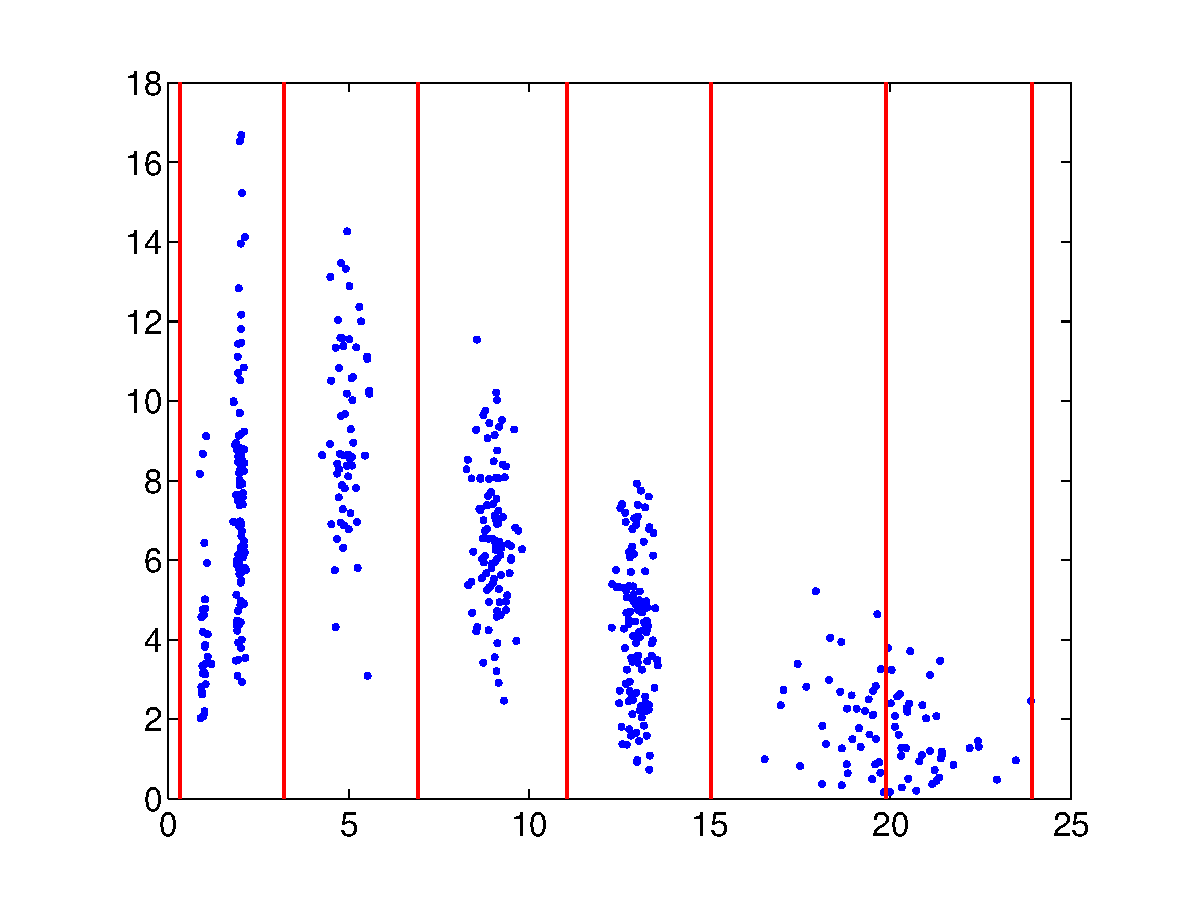
\includegraphics[scale=0.35, trim = 18mm 9mm 15mm 0, clip ]{inputs/2a.eps}
\label{potEx:subfig1}
}
\subfigure[Colored lines: terms from each bin that contribute to make up $\phi$. Black dashed line: $\phi$, the complete data density function (it's mostly behind the colored lines except for in the vicinity of x=20).  ]{
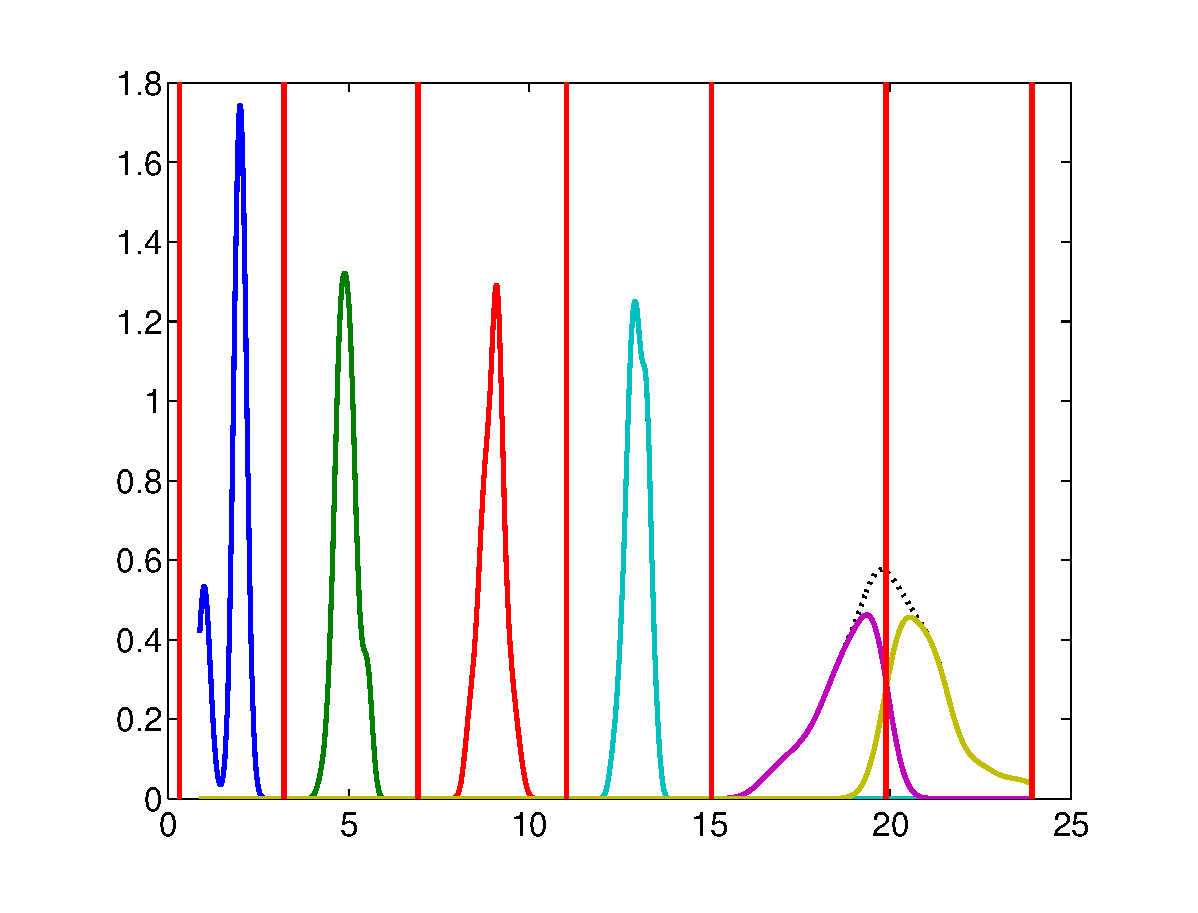
\includegraphics[scale=0.35, trim = 16mm 9mm 15mm 0, clip ]{inputs/2b.eps}
\label{potEx:subfig2}
}
\subfigure[Binning with pentality term.]{
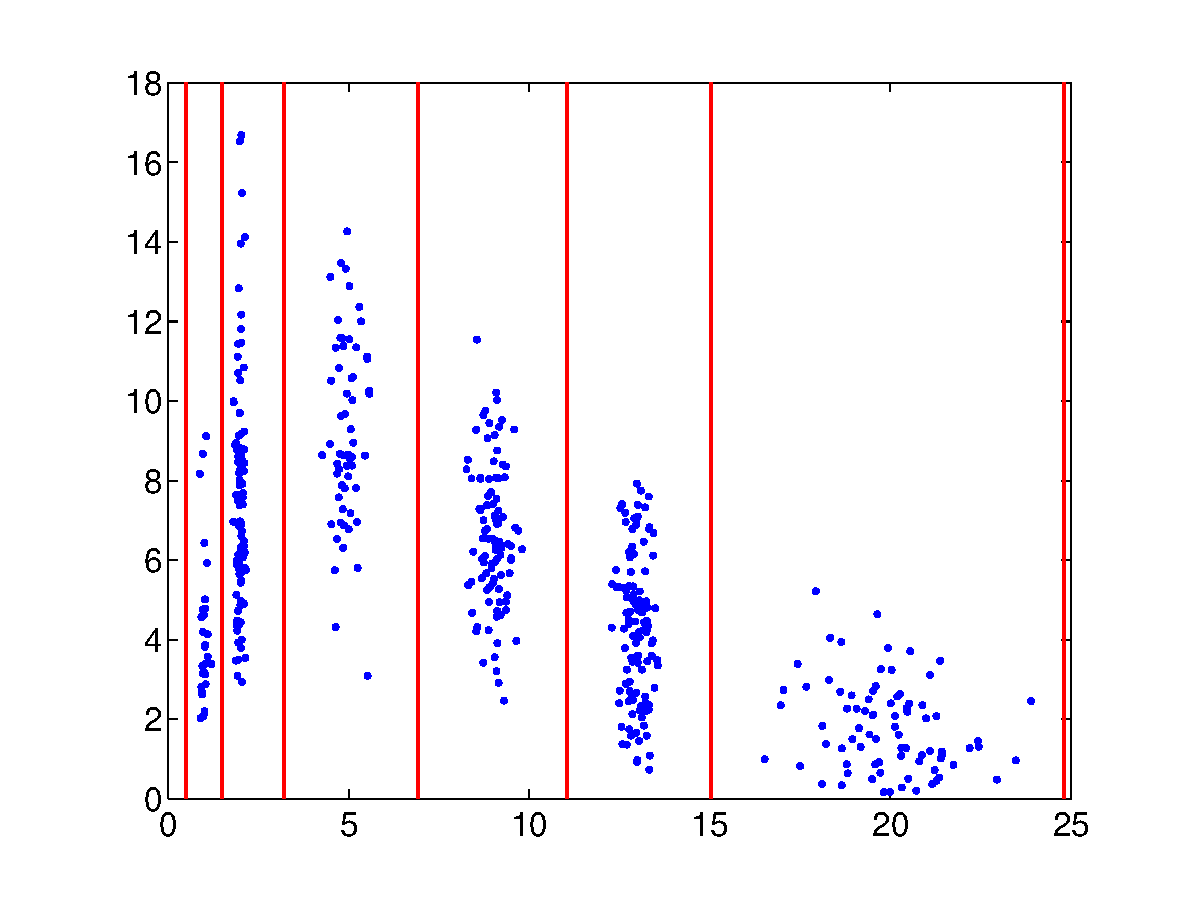
\includegraphics[scale=0.35, trim = 18mm 9mm 15mm 0, clip ]{inputs/2c.eps}
\label{potEx:subfig3}
}
\caption[]{The effect of the potential function}
\label{potEx}
\end{figure}

\subsection{Scale factor $\alpha$}
The method to minimize (\ref{eq:objectiveFunction1}) can be written in short notation as
\begin{equation}
	\operatorname{Minimize} W + \alpha\Phi
	\label{eq:Method1}
\end{equation}
Note that by the definition of $\Phi$, having $K$ clusters of data with a decent pre-binning with $K$ bins, the local maximums of $\phi$ will be approximately of size 1. This can for example be seen in Figure \ref{potEx:subfig2}. To relate $W$ with $\Phi$ in the objective function the scale factor $\alpha=C\max_k{W_{0,k}}$ was used with $C$ beeing a constant. Empircal testing suggested $C=7.8$ for best results. The resulting binning of the final method can be seen in Figure \ref{potEx:subfig3}.


\subsection{Effect of the data density function}
%Tycker det här stycket känns lite halvdant
In Figure \ref{potEx} the effect of the data density function is illustrated. Without the data density function only the K-means objective function is considered. In Figure \ref{potEx:subfig1} the last cluster has much spread and K-means undesirably splits it into two bins. Applying the data density function on this binning gives a contribution to the objective function which penalizes the algorithm in placing the bin on that location (Figure \ref{potEx:subfig2}). Instead the bin is placed so that the first two clusters are separated (Figure \ref{potEx:subfig3}). The binning now  better corresponds to the desired binning characteristics of the modelers.
\



\section{Minimization method \& estimation of the number of bins}
The algorithm seeks to place out $K$ bins in a way such that the objective function is minimized. To avoid having initial bins violating the minimal number of data points in each bin constraint, the equal size method with the same constraint is used as the initial guess. It can be computed very fast and gives a good starting point. We have not noticed any difference in result using different initial guesses, however an initial value that resembles the final result makes the algorithm converge faster.

\par
To make the minimization algorithm more efficient, instead of minimizing the within-cluster variability $W$, the total variability $T$ minus the between cluster variabiliy $B$ was minimized. This simplification is possible since the total variability equals $T=W+B$ \cite{Yan}. The different variabilities are defined as

\begin{equation}
	T = \sum_{i=1}^n  (x_{i} - \bar{x})(x_{i} - \bar{x})^T
	\label{eq:T}
\end{equation}

\begin{equation}
	W = \sum_{k=1}^K \sum_{l = 1}^{n_k} (x_{kl} - \bar{x}_k)(x_{kl} - \bar{x}_k)^T
	\label{eq:W}
\end{equation}

\begin{equation}
	B = \sum_{k=1}^K n_k (\bar{x}_k - \bar{x})(\bar{x}_k - \bar{x})^T,\
	\label{eq:B}
\end{equation}

\begin{equation}
 	\bar{x} = \frac{1}{n} \sum_{i=1}^n x_i.
\end{equation}

and $x_{kl}$ is the $x$ value in the $l:th$ point in bin $k$ and $n_k$ is the number of points in bin $k$.

\begin{algorithm}
	\caption{Minimization Algorithm}
	 Continue optimization until the following stop criteria is fulfilled: 
	\begin{enumerate}
		\item No bin boundary can favorably be moved between its two neighbors.  
		\item No bin boundary can favorably be moved in-between any two other bin boundaries. 
	\end{enumerate}
	{\bf Part I of the optimization}\\
	Try moving the bin edges one by one within its two neighbors to decrease the objective function. \\
	Step 1: \\
	Choose the bin edge that gives the biggest decrease
       (or smallest increase) when being moved one step to the left or right.
     Then calculate the objective function for every possible position between the two neighbour 
       bin edges and move it where it is lowest.\\
	Step 2: \\
	   Mark the moved bin edge as updated so that it can't be moved again unless another edge is moved first.\\
	   Step 3: \\
	   If a bin edge has been moved, update the neighboring bin edges so that they can be moved again.  \\\\
	   
	    {\bf Part II of the optimization}\\
	    Try taking out the bin edges one by one and placing them in between two other bin edges to decrease the objective function \\
	    Step 1: \\ 
	    Calculate the increase in the objective function for removing any of the bin edges. Also calculate the decrease in the objective for adding an extra between bin edge between any two consecutive bin edges.\\
	    Step 2: \\
	     If there is any move of a boundary that results in a decreased objective function, perform the movement that results in the largest decrease and go back to PART I, else stop. 


\label{Minimizer}
	   
\end{algorithm}
\newpage
\subsection{Choosing the number of bins}
Determining the number of bins in the data is an important problem. It affects the resolution of the VPC. In some cases the number of bins is obvious. In general this is not the case and the number of bins must be estimated by the user of the VPC based on some prior knowledge of the data or estimated somehow. Since we want a fully automatic binning we need a method that does this for us.
\par
A simple and direct strategy would be to use our objective function (eq. \ref{eq:Method1} ) not only to place our bins but also to estimate the number of bins. For our two methods presented in the previous section, we then get the following: 

\begin{equation}
	  \underset{K}{\operatorname{arg\,min}} \,\, W(K) + \Phi(K)
\end{equation}

After trials we could conclude that this way of estimating the number of bins works well when incorporating y while it has a tendency to underestimate the number of bins when only considering the independent variable. 
\par
There exists a variety of methods to estimate the number of bins. In an article written by G. Milligan \& M. Cooper \cite{Milligan} different methods of estimating the number of clusters have been evaluated. The method that in general outperformed the others was the Calinski and Harabaszs method,
\begin{equation}
	\underset{K}{\operatorname{arg\,max}}\,\, \frac{B/(K-1)}{W/(n-K)}.
\end{equation}
where B is defined in eq. \ref{eq:B}.

Tests of this method gave good results on most but not all data sets when using Method 1. It had a tendency to overestimate the number of bins.
\par
Because our first approach to use the objective function had a tendency to underestimate the number of bins and the Calinski \& Harbaszs method had the opposite tendency the quotient was tested:

\begin{equation}
	\underset{K}{\operatorname{arg\,max}}\,\, \frac{B/(K-1)}{W/(n-K)} / (W + \alpha\Phi).
	\label{eq:estimateK}
\end{equation}

In many of the cases where the data was well separated both the objective function and the Calinski \& Harbaszs method gave the same result which coincides with the results of eq. (\ref{eq:estimateK}). In the cases where they gave different results eq. (\ref{eq:estimateK}) weighted the two methods in a way that the estimation of the number of bins gave a good result on the data sets used for method development.

\begin{thebibliography}{99}
	\bibitem{Sonehag} Christian Sonehag, Niklas Olofsson and Rasmus Simander, {\em Automatic binning in visual predictive checks}, Feb 2012, Undergraduate project http://www.it.uu.se/edu/course/homepage/projektTDB/ht11/project4/Report\_ht11\_04.pdf
 \bibitem{Lavielle} M. Lavielle, K. Bleakley, {\em Automatic data binning for improved visual diagnosis of pharmacometric models}, June 9, 2011
 \bibitem{GaussianKernel} Silverman, B.W. {\em Density Estimation for Statistics and Data Analysis}, 1998.
 \bibitem{KMeans} J.B. MacQueen. Some methods for classification and analysis of multivariate observations. {\em Proceedings of 5th Berkeley Symposium on Mathematical Statistics and Probability}, pages 281-297. University of California Press, 1967.
 \bibitem{Milligan} G. Milligan, M. Cooper, {\em An examination of procedures for determining the number of clusters in a data set}, Psychometrika-vol. 50, no 2, 159-179. June 1985
 \bibitem{Yan} M. Yan, {\em Methods of Determining the Number of Clusters in a Data Set and a New Clustering Criterion}, November 2005
\end{thebibliography}


\appendix
\section*{Appendix}
\section{K-means algorithm}
\begin{algorithm}
	\caption{K-means Algorithm}
	Given an initial set of $k$ means $m = (m_1^1, m_2^1, ..., m_k^1)$ the algorithm proceeds by alternating between two steps:
	\\ 
	\\
	{\bf Assignment step: } Assign each observation to the cluster with the closest mean.
	$S_i^{(t)} = \{ x_p : || x_p - m_i^{(t)} || \leq || x_p - m_j^{(t)} || \,\, \forall \, 1 \leq j \leq k \}$ 
	\\
	\\
	{\bf Update step: } Calculate the new means to be the centroid of the observations in the cluster.
	$m_i^{(t+1)} = \frac{1}{| S_i^{(t)} |} \sum_{x_j \in S_i^{(t)}} x_j$
	\\
	\\
	{\bf Repeat: } Until no changes can be made in the assignment step.


\label{kmeans}
	   
\end{algorithm}

\end{document}
